\section{Benefits of Tiny Tasks}
\label{sec:benefits}
\eat{Tiny tasks benefit data center workloads by providing inherent elasticity:
fine-grained units of work can be dynamically allocated to machines as
resources become available, eliminating stragglers and issues of data skew,
and allowing jobs to use available resources without sacrificing fairness
when new jobs are submitted.}

Tiny tasks benefit datacenter workload by increasing the amount of elasticity
available to the scheduler, as resources are occupied for a very small duration,
resources can be allocated to fine grained tasks at a very fine granularity. This 
allows resources to be dynamically reallocated to jobs, eliminating problems caused
by straggling tasks, data skew, and allowing greater cluster utilization without
sacrificing request latency.

\subsection{Handling of skew and stragglers}
Prior studies~\cite{ananthanarayanan2010reining,zaharia2008improving} have noted that
task lengths in dataparallel workloads are highly variable, and the negative impact outlier
tasks have on job completion time. Outliers occur for a variety of reasons, including an
uneven division of work across tasks (data skew), the state of a machine, network congestion
and others. 

Tiny tasks help mitigate the effect of outliers in two ways: firstly splitting total work
across a larger set of tasks more evenly partitions records across tasks, reducing data skew;
secondly, individual tasks can be moved in response to slow machines, network congestions, or
other cluster conditions, and run on other, faster machines.

To quantify these benefits, we start by simulating the effects of even load balancing. We obtained
a trace from a cluster at Facebook, and simulated these effects by evenly spreading total task time
for a job across all the slots that were originally assigned to the job. Our results are shown in
Figure~\ref{fig:binpacked}, where it can be seen that about $30\%$ of small jobs, and $60\%$ of 
large tasks benefit from more evenly spreading the load. 

\begin{figure}[t]
\centering
\hspace{2ex}
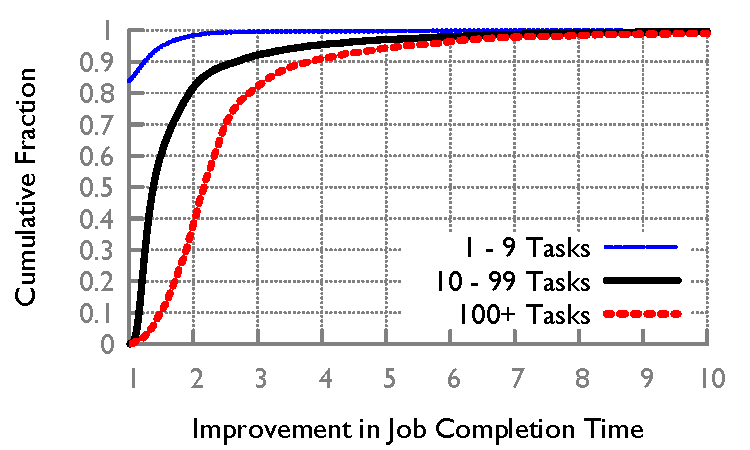
\includegraphics[width=0.5\textwidth]{figures/binpacked1-sep}
\vspace{-4ex}
\caption{Ideal improvement from binpacking tasks.}
\vspace{-2ex}
\label{fig:binpacked}
\end{figure}

\eat{Figure~\ref{fig:sparkskew} demonstrates the improvement offered by tiny tasks on a Spark MapReduce job with data skew and machines that exhibited a random 5x performance variance.
With tiny tasks, Spark is able to mitigate both skew and stragglers without explicit knowledge of machines' speeds or records' processing costs.}

We next analyzed the straggler mitigation benefits offered by tiny tasks. Our analysis was based on running
Spark jobs on $50$ m1.medium EC2 machines, explicitly introducing data skew, and introducing random delays
so that task times varied by over 5x. We vary the number of tasks launched (and therefore the data that
needs to be processed per task) and show (Figure~\ref{fig:sparkskew}) both improvements in job time,
and reduction in task variance, without providing the scheduler with any additional information.

\begin{figure}[t]
\centering
\hspace{2ex}
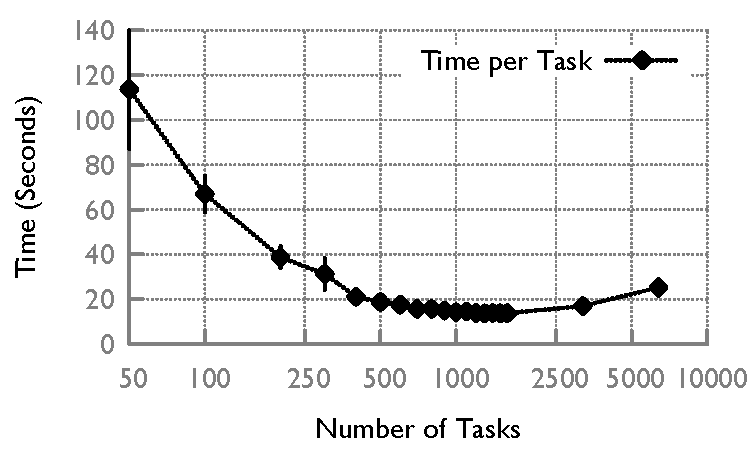
\includegraphics[width=0.5\textwidth]{figures/spark-skew-results}
\vspace{-4ex}
\caption{Improvement from using tiny tasks in the presence of skew and heterogeneous machines. Error bars depict standard deviation.}
\vspace{-2ex}
\label{fig:sparkskew}
\end{figure}



\subsection{Response Time}
Sharing a cluster between interactive and batch jobs requires that one to make a
tradeoff between responsiveness and utilization. If a cluster is highly utilized
an interactive request must wait for running tasks to complete before it can be
serviced, while reserving slots for interactive jobs results in lower utilization. Tiny
tasks allow one to pick a point between these two extremes. Since tasks run for a much
shorter duration, batch jobs can use a larger percentage of the cluster, increasing
utilization, while simultaneously guaranteeing that interactive jobs must wait for 
a reasonably short time before being serviced.

In Figure~\ref{fig:kay} we show these gains in responsiveness using a simulation. Our
simulation measures the time a job must wait before the first of its tasks starts running
at varying utilization values.
